1\chapter{Numerical domains III: Pentagons}
\section{General}
\begin{itemize}
\item Pentagon domain is a reduced product of two domains: Interval ($c \leq x \leq d$) and Strict Upper Bounds (SUB) ($x < y$)
\item Quadratic space complexity
\item Quadratic time complexity
\item Useful for checking array out of bounds error
\begin{itemize}
\item interval component takes care of index underflow ($index \geq 0$)
\item the SUB component takes care of index overflow ($index < array.length$)
\end{itemize}
\end{itemize}
\section{Domain of Strict Upper Bounds (SUB)}
\begin{itemize}
\item for each variable $x$ store the list $s(x)$ of all other variables $y$ s.t. $x<y$
\item SUB domain: $\{S^S, \sqsubseteq_S,\sqcup_S,\sqcap_S,\bot_S,\top_S\}$
\item $\bot_S \iff \exists x,y$ s.t., $y \in s(x) \wedge x \in s(y)$
\item $S$ is the set of all SUB inequalities, $S^S=S \cup \{\bot_S\}$
\item $\top_S \iff \forall x,s(x)=\emptyset$
\end{itemize}
\section{Formalization}
\begin{itemize}
\item $s_1 \subseteq_S s_2 \iff \forall x, s_1(x) \supseteq s_2(x)$
\item $s_1 \sqcup_S s_2 = \forall x.s_1(x) \cap s_2(x)$
\item $s_1 \sqcap_S s_2 = \forall x.s_1(x) \cup s_2(x)$
\item $s_1 \nabla_S s_2 = \forall x.s_1(x) \subseteq s_2(x) ? s_2(x) : \emptyset$
\item Closure is not performed to avoid cubic complexity. 
\begin{itemize}
\item therefore no galois insertion 
\item Domain loses precision for various operators
\end{itemize}
\end{itemize}
\noindent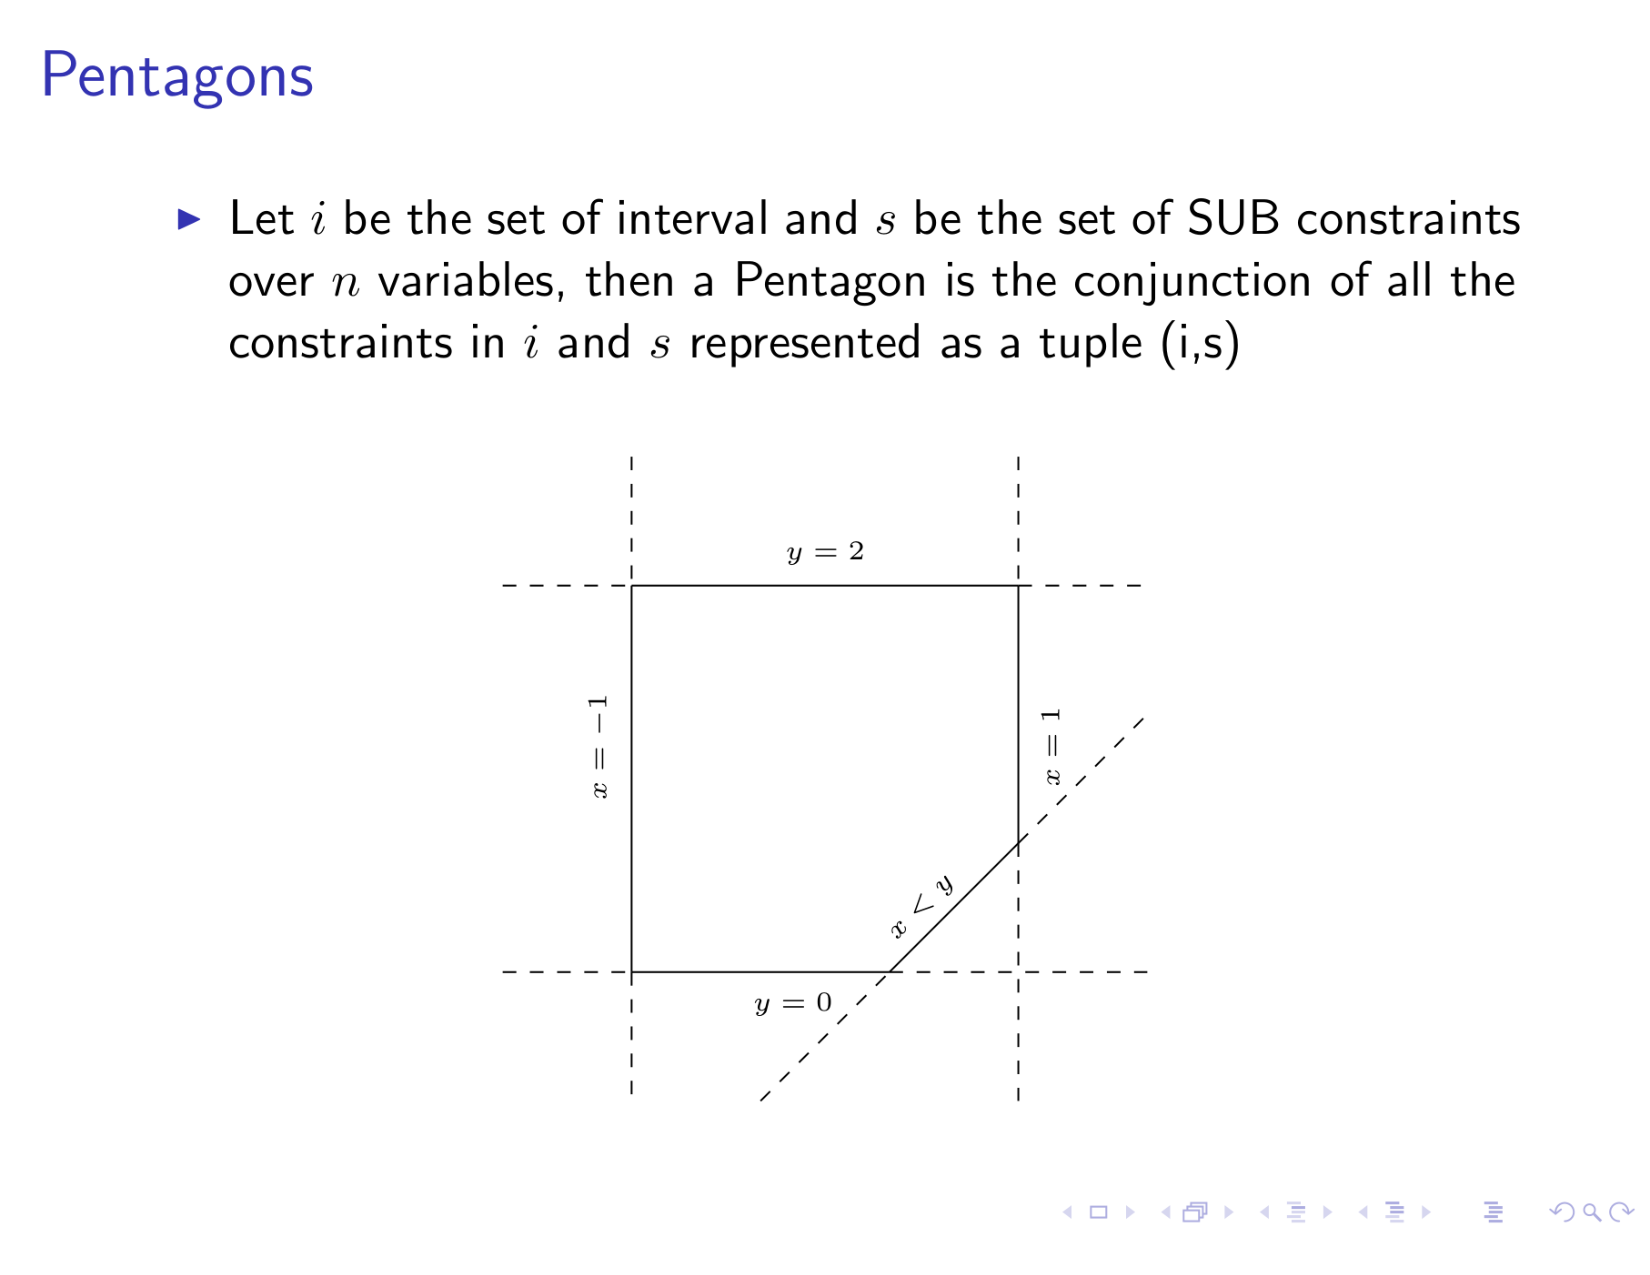
\includepdf[,landscape=true,nup=2x2,pages={-}]{pages/pentagon.pdf}
